\documentclass[10pt,a4paper]{article}
\usepackage[utf8]{inputenc}

% Define the page margin
\usepackage[margin=3cm]{geometry}

% Better typography (font rendering)
\usepackage{microtype}

% Math environments and macros
\usepackage{amsmath}
\usepackage{amsfonts}
\usepackage{amssymb}
\usepackage{amsthm}

% Define \includegraphics to include graphics
\usepackage{graphicx}

% Draw graphics from a text description
\usepackage{tikz}

% Syntax highlighting
\usepackage{minted}

% Set global minted options
\setminted{linenos, autogobble, frame=lines, framesep=2mm}

% Import the comment environment for orgtbl-mode
\usepackage{comment}

% Do not indent paragraphs
\usepackage{parskip}

\title{Databases, Sheet 10}
\author{Marten Lienen (03670270)}

\begin{document}

\maketitle

\section*{Exercise 1}

\subsection*{Part a)}

Eine TID ist die ID eines Datensatzes innerhalb einer Tabelle.
Ihr Einsatz lohnt sich z.B., wenn man mehrere B-Baum-Indizes für eine Tabelle haben möchte, weil man Suchergebnisse auf verschiedenen Attributen einschränken will.

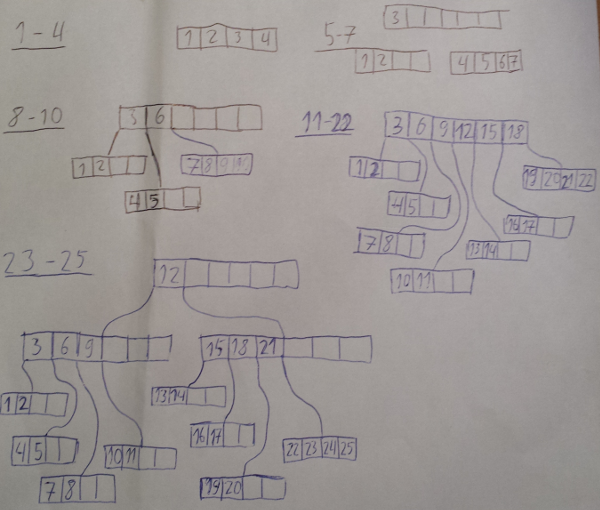
\includegraphics[width=\textwidth]{sheet-10/exercise-1-a}

\subsection*{Part b)}

Man durchläuft den Baum und gibt alle Datensätze zurück, deren Schlüssel zwischen 5 und 15 liegt.
Wenn dies auf ganze Teilbäume zutrifft, kann man die Suche optimieren, weil man dann schon weiß, dass es für alle Datensätze in diesem Teilbaum zutrifft.

\section*{Exercise 2}

Jeder Eintrag inklusive Schlüssel ist also ca. $100 + 8 = 108$ Byte groß.
Die Speicherplatzanforderung der Verweise auf Kinder kann man wohl als ca. $8$ Byte annehmen.
Ein Knoten eines B-Baums des Rangs $k$ braucht also maximal $2k \cdot 108 + (2k + 1) \cdot 8 = 232k + 8$ Byte.
Dieser Wert soll jetzt bezüglich $k$ maximiert werden, sodass der Wert jedoch kleiner als $16000$ bleibt.
\begin{equation*}
  232k + 8 \le 16000 \Leftrightarrow 232k \le 15992 \Leftrightarrow k \le \frac{15992}{232} \approx 68.93
\end{equation*}
Also ist $k = 68$ der maximale Wert, mit dem die Blöcke noch auf einer Seite bleiben und gleichzeitig die Auslastung optimiert wird.

Ein solcher Baum der Höhe $h$ kann maximal $2k + (2k + 1) * 2k + (2k + 1)^{2} * 2k + \dots = 2k \sum_{i = 0}^{h} (2k + 1)^{i}$ Elemente aufnehmen.
Nennen wir diese Anzahl $n$.
Anwendung der Partialsummenformel für geometrische Reihen ergibt $n = 2k \cdot \frac{1 - (2k + 1)^{h + 1}}{1 - (2k + 1)} = (2k + 1)^{h + 1} - 1$.
Durch Auflösen nach $h$ können wir nun die minimal erforderliche Höhe berechnen, die notwendig ist, um $n$ Datensätze aufzunehmen.
\begin{equation*}
  h = \log_{2k + 1}(n + 1) - 1
\end{equation*}
In diesem konkreten Fall ergibt sich eine minimale Höhe von $h = \log_{133}(10000000001) - 1 \approx 3.7$.
Eine Höhe von $h = 4$ ist also ausreichend.

\section*{Exercise 3}

Als Hashfunktion benutzen wir, wie in der Vorlesung, die umgekehrte Binärdarstellung der Kundennummer.
Dabei ergeben sich die Hashes

% BEGIN RECEIVE ORGTBL exercise-3
\begin{tabular}{rrr}
KundenNr & Binär & Hash\\
\hline
10 & 1010 & 010100\\
18 & 10010 & 010010\\
25 & 11001 & 100110\\
30 & 11110 & 011110\\
40 & 101000 & 000101\\
45 & 101101 & 101101\\
\end{tabular}
% END RECEIVE ORGTBL exercise-3
\begin{comment}
#+ORGTBL: SEND exercise-3 orgtbl-to-latex :splice nil :skip 0
| KundenNr |  Binär |   Hash |
|----------+--------+--------|
|       10 |   1010 | 010100 |
|       18 |  10010 | 010010 |
|       25 |  11001 | 100110 |
|       30 |  11110 | 011110 |
|       40 | 101000 | 000101 |
|       45 | 101101 | 101101 |
\end{comment}

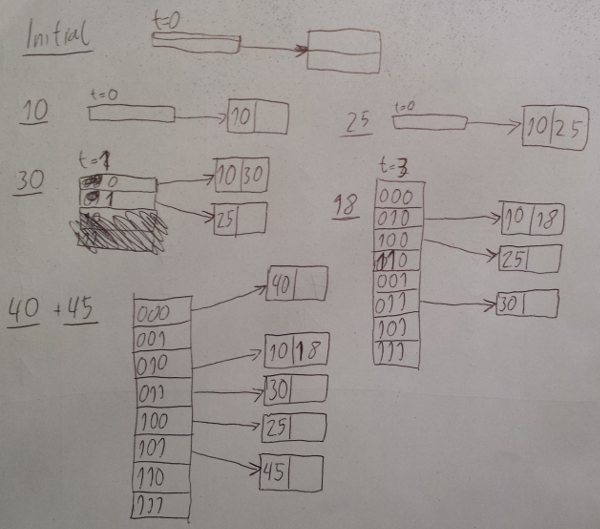
\includegraphics[width=\textwidth]{sheet-10/exercise-3}

\section*{Exercise 4}

Bei globaler Tiefe $t$ hat das Directory $2^{t}$ Einträge, einen für jede mögliche Kombination der ersten $t$ Bits.
Für einen Bucket der Tiefe $t'$ sind jedoch nur die ersten $t'$ Bits relevant.
Deshalb zeigt für jede Kombination der $t - t'$ überschüssigen Bits ein Indexeintrag auf diesen Bucket.
In der Summe sind dies $2^{t - t'}$.

\end{document}
